\documentclass{article}
\usepackage[utf8]{inputenc}
\usepackage{titling}
\usepackage{graphicx}
\usepackage{xcolor}
\usepackage[colorlinks=true,linkcolor=darkgray, urlcolor =gray]{hyperref}
\usepackage[spanish]{babel}
\DeclareUnicodeCharacter{301}{~}
\usepackage{url}
\usepackage{graphicx}
\usepackage{caption}
\usepackage{subcaption}
\DeclareUnicodeCharacter{202F}{\,}


\title{Comercio electrónico con Prestashop}
\author{Álvaro Fernández Palma\\ Alina Altynguzhina\\ Iman Hasnaouia Meskini\\ Cristina Díaz García}
\date{Noviembre 2018}

\renewcommand\maketitlehooka{\null\mbox{}\vfill}
\renewcommand\maketitlehookd{\vfill\null}


\begin{document}

\addcontentsline{toc}{section}{Índice general}

\begin{titlingpage}
\maketitle

\begin{flushleft}

\includegraphics[scale=0.4]{images/prestashop.png} 
\end{flushleft}

\end{titlingpage}

\newpage

\tableofcontents

\newpage

\section{Plan de Trabajo}

\subsection{Tareas} 

\textbf{Iman:} Relación con la teoría, funcionalidades, personalización y parte opcional. 

\textbf{Alina:} Conclusiones. 

\textbf{Álvaro:} Funcionalidades y conclusiones. 

\textbf{Cristina:} Presentación, memoria e integración. 


\section{Introducción}

Prestashop es una plataforma open source con la que crear tiendas online para poder comerciar con nuestros productos. En las siguientes páginas analizaremos diferentes aspectos técnicos, como sus funcionalidades, la personalización o la integración que pueda tener con otras aplicaciones.

\section{Funcionalidad de prestashop}



\subsection{Dashboard}

PrestaShop es una plataforma de carrito de compras gratuita que permite a pequeñas y grandes empresas crear y gestionar una tienda en línea. Se trata de un gestor de contenidos dinámico pensado para construir desde cero tiendas con software 100\% gratuito, que además puede ser alimentado con temas y módulos gratuitos o desarrollados por profesionales bajo licencias comerciales. Desde 2007, fecha en la que PrestaShop vio la luz, cada vez más negocios online utilizan esta plataforma de e-commerce para gestionar la venta de productos físicos o digitales, existiendo en la actualidad más 250.000 tiendas funcionando con este CMS de origen francés. Trabaja con innumerables pasarelas de pago entre las que destacan Paypal, Authorize.net, Google Checkout, Skrill, Moneybookers, Klarna, Redys/Servired/Sermepa, etc. Pero lo que caracteriza de verdad a esta plataforma e-commerce es la facilidad, ya que en cuestión de minutos es posible tener en la red una tienda online sin demasiados conocimientos informáticos.

\subsection{Pedidos}

En la pestaña de pedidos se encuentra la funcionalidad de administrar los pedidos en la tienda.

\begin{center}
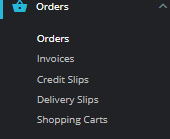
\includegraphics[scale=0.4]{images/pedidos.png}
\end{center}

Lo primero que se puede ver es la información de los pedidos en proceso. Se muestra la información del producto, la información del cliente y la información referente al estado del producto (En proceso de pago, cancelado, enviado, etc.).

\begin{center}
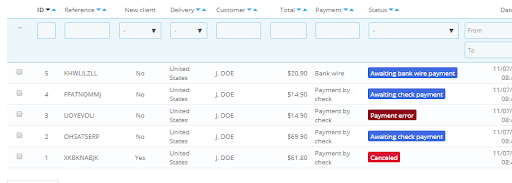
\includegraphics[scale=0.8]{images/facturas.png}
\end{center}

Hay opciones que permiten administrar las facturas. Se puede enviar automáticamente la factura al cliente cuando este efectúa una compra si el administrador lo desea, editar el formato de la factura, generar automáticamente un pdf con todas las facturas y ordenarlas según el status de los pedidos.
Otra funcionalidad bastante interesante es la pestaña de Carritos de Compra, en la cual se pueden visualizar todos los carritos de compra de cada cliente junto con la información del cliente, la fecha, si se ha efectuado la compra de ese carrito o si se ha abandonado, la cantidad que se ha pagado o se pagaría si se hubiese efectuado la compra, etc.

\begin{center}
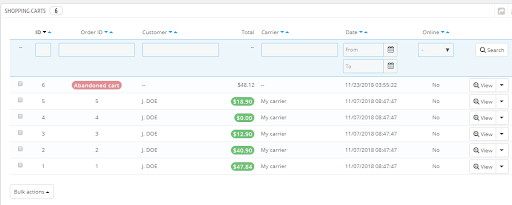
\includegraphics[scale=0.8]{images/facturas2.png}
\end{center}

\subsection{Catálogo}

En la pestaña de catalogos, se puede modificar el catálogo. Se pueden introducir productos, categorías, monitorizar, editar los atributos y características, ficheros, descuentos y stocks.

\begin{center}
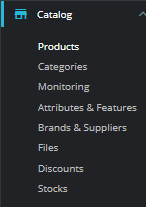
\includegraphics[scale=0.8]{images/catalogo.png}
\end{center}

\begin{center}
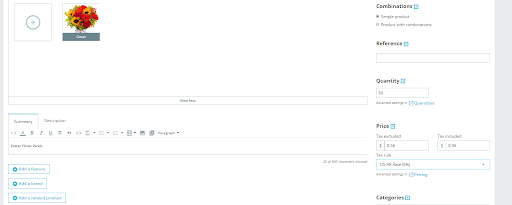
\includegraphics[scale=0.8]{images/ejemplo.png}
\end{center}

Al introducir un producto, hay una parte donde se pueden poner imágenes, introducir el precio del producto, nombre, descripción, etc. Y también hay otras pestañas en las que se puede editar de manera más específica las cantidades de producto que hay en el almacén, las modalidades de envío y características del paquete (tamaño, peso), editar de manera más específica los precios de los productos teniendo en cuenta los impuestos, configuración del SEO para hacer la búsqueda más personalizada.

\begin{center}
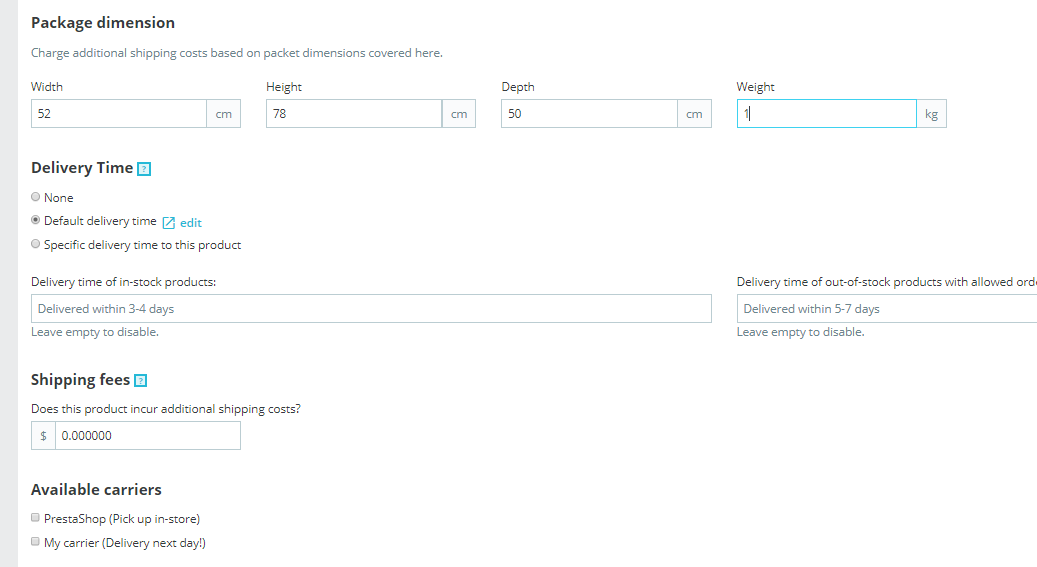
\includegraphics[scale=0.4]{images/paquete.png}
\end{center}

\subsubsection{Categorías}

En la pestaña de categorías se pueden crear o eliminar categorías para clasificar los productos, como ropa, accesorios, vestidos, camisetas, mochilas, etc.

\begin{center}
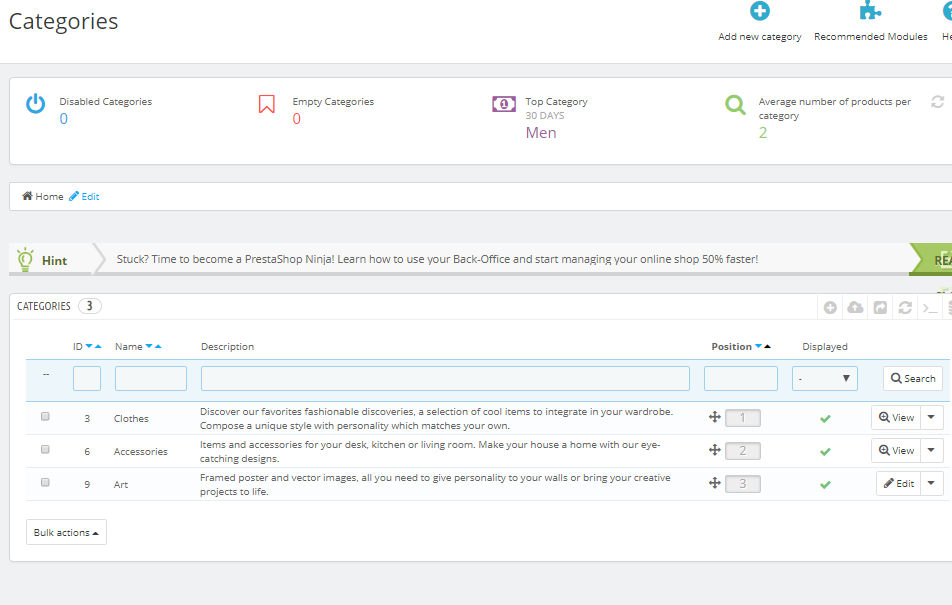
\includegraphics[scale=0.4]{images/categorias.png}
\end{center}

\subsubsection{Monitorización}

En la pestaña de monitorización se puede monitorizar el catálogo, es decir, añadir o quitar visibilidad a productos, categorías, productos dentro de categorías, visualizar las categorías vacías o productos combinados en el cual haya falta de stock, productos sin imágenes, sin precio, etc. Esto permite corregir errores a la hora de crear categorías y productos cuando se olvida añadir imagen, descripción a un producto o cuando se añade una categoría y no se le añaden productos, permitiendo así una mayor limpieza de la tienda online.

\begin{center}
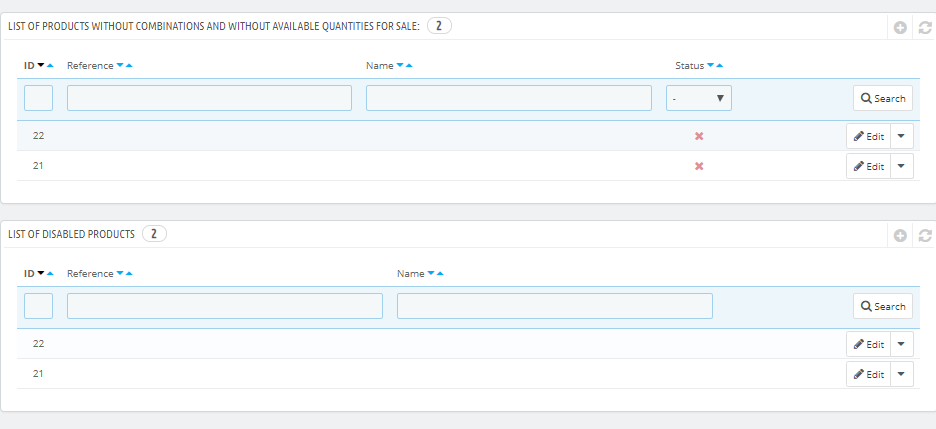
\includegraphics[scale=0.4]{images/monitoring.png}
\end{center}

\subsubsection{Atributos y características}

En la prestaña de atributos y características se pueden modificar estos. Si tenemos una característica como “Talla” y nuestra tienda abarca tallas dentro del conjunto {“S”,”M”,”L”}, simplemente a ese atributo se le añaden esos valores, y en el momento que haya que aumentar o disminuir  ese atributo por aumento o disminución de tallas, solo hay que añadir o quitar valores. Y lo mismo sería para las características.

\begin{center}
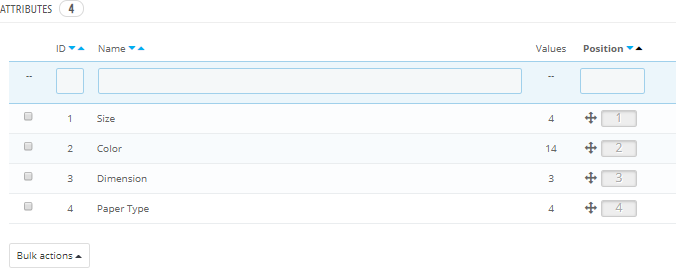
\includegraphics[scale=0.4]{images/atributos.png}
\end{center}

\subsubsection{Marcas y proveedores}

En la pestaña de marcas y proveedores  se pueden añadir o eliminar marcas de los productos que se venden en nuestra tienda y sus direcciones  o proveedores de productos que vendemos. 

\subsubsection{Descuentos}

En la pestaña de descuentos se pueden añadir o quitar descuentos para productos, automatizándose así el precio nuevo del producto.

\subsubsection{Stock}

En la pestaña de stock, se puede administrar el stock de la tienda, en el que se muestra si un producto está disponible para la venta según el número de unidades del producto físicas disponibles y el número de unidades reservadas. También se muestran los datos del proveedor.

\begin{center}
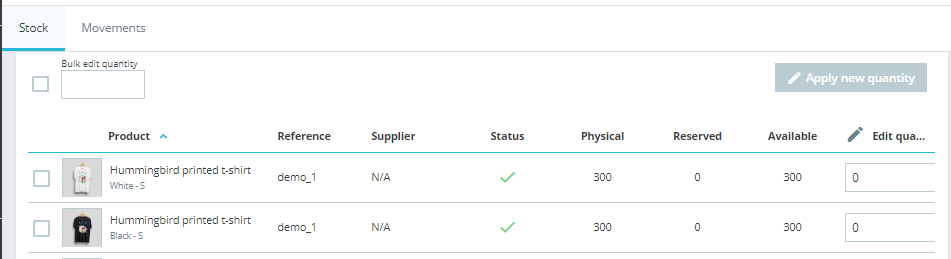
\includegraphics[scale=0.4]{images/stock.png}
\end{center}

\subsection{Clientes}

\begin{figure}[h!]
        \raggedright
        \begin{subfigure}[!]{0.2\textwidth} 
            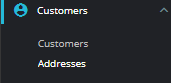
\includegraphics[width=\textwidth]{images/customers.png}
        \end{subfigure}       
        \begin{subfigure}[!]{0.7\textwidth} 
            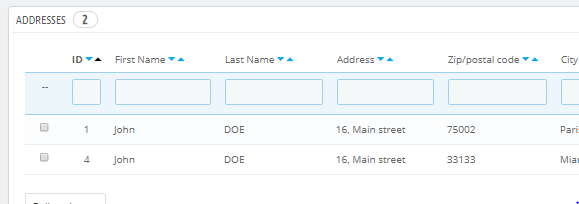
\includegraphics[width=\textwidth]{images/cliente.png}
        \end{subfigure}
    \end{figure}

En la pestaña de clientes se pueden observar los clientes de la tienda, sus datos y direcciones, pudiendo utilizarse esta información para el futuro envío de productos a estos clientes, personalizar la tienda según sus datos, etc.

\subsubsection{Servicio al Cliente}

La pestaña de servicio al cliente es la funcionalidad de Prestashop que permite toda la comunicación con el cliente antes, durante y después de las transacciones de compra. Hay una visualización general donde se ven el número de hilos abiertos, cerrados, pendientes, mensajes de clientes, mensajes de empleados e hilos no leídos.

\begin{center}
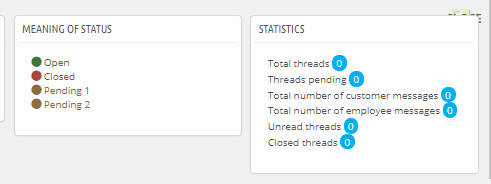
\includegraphics[scale=0.6]{images/cuse.png}
\end{center}

Hay opciones de contacto y opciones de servicio al cliente. En las opciones de contacto se configura el formato del mensaje que se le envía al cliente. En las opciones del servicio al cliente se añaden o quitan funciones a los clientes y empleados, como permitir o no borrar mensajes, la posibilidad de poder crear hilos, etc.

\begin{center}
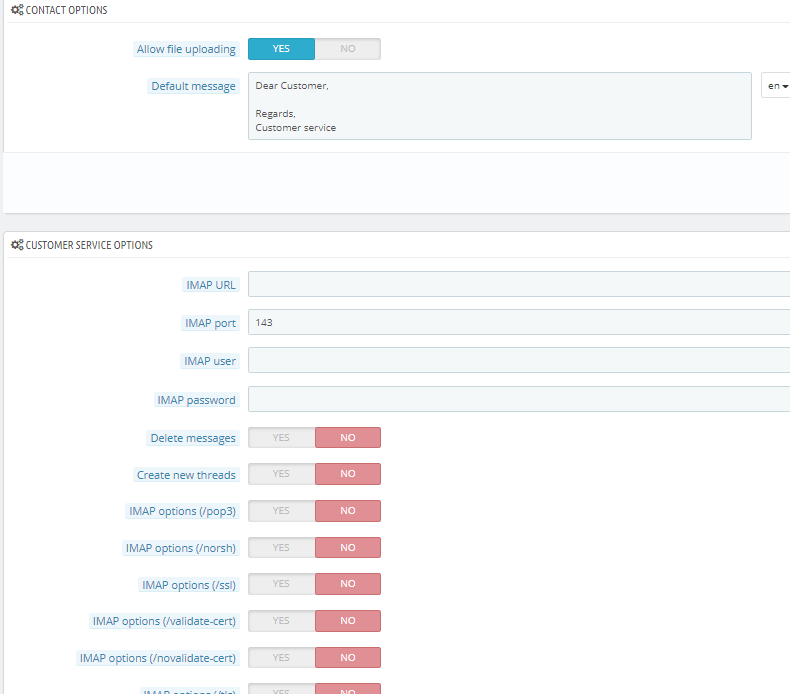
\includegraphics[scale=0.4]{images/opciones.png}
\end{center}

\subsubsection{Mensajes del pedido}

En la pestaña de mensajes del pedido  se administran los mensajes relacionados con un pedido, por ejemplo, enviar al cliente un mensaje diciendo que su pedido, por falta de stock, no se ha podido enviar, o que se ha enviado el producto, por ejemplo.

\begin{center}
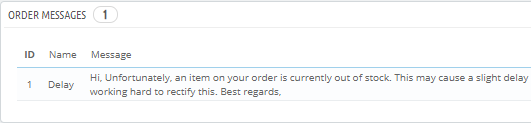
\includegraphics[scale=0.6]{images/mensajes.png}
\end{center}

\subsubsection{Devoluciones}

En la pestaña de devoluciones, se administra el tema de las devoluciones de productos que los clientes ya han comprado, en la cual se muestran los datos del producto y las opciones de las devoluciones, como permitir o no la devolución de productos en nuestra tienda.

\subsubsection{Estadísticas}

En estadísticas se observan estadísticas generales de las ventas de la tienda, permitiendo de esta manera una visualización de datos bastante intuitiva y sencilla de interpretar.

\begin{center}
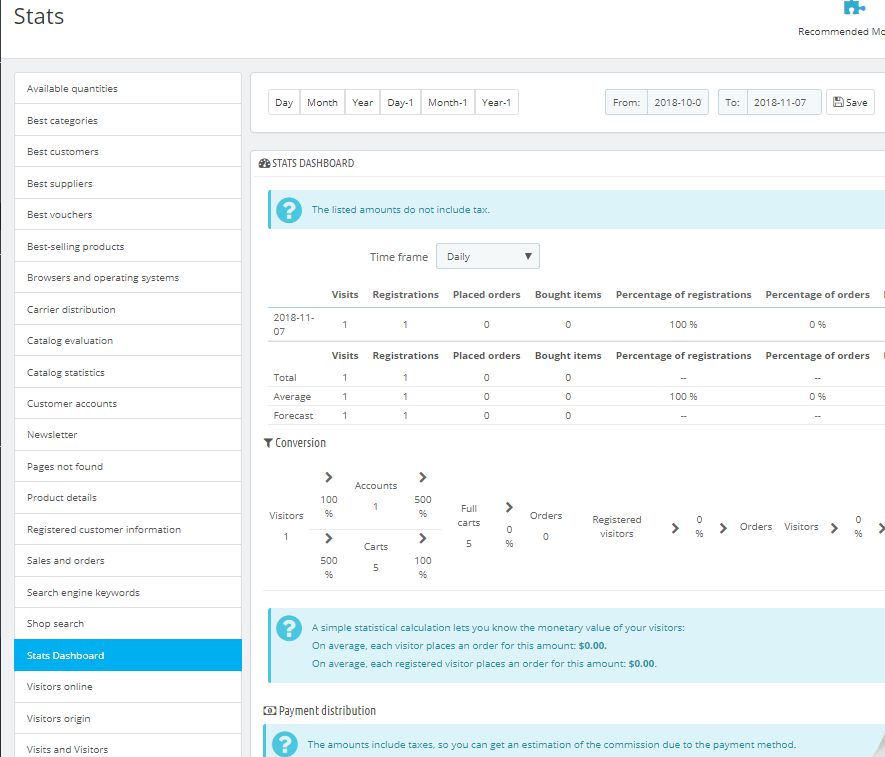
\includegraphics[scale=0.3]{images/stats.png}
\end{center}

\subsection{Módulos}

Funcionalidad que permite administrar los módulos habilitados, deshabilitados y los que se tienen instalados. Tiene un panel de búsqueda y recomendación de módulos que se pueden añadir a nuestra tienda y  un panel de notificaciones que nos hace saber si necesitamos actualizar o configurar algún módulo.

\begin{center}
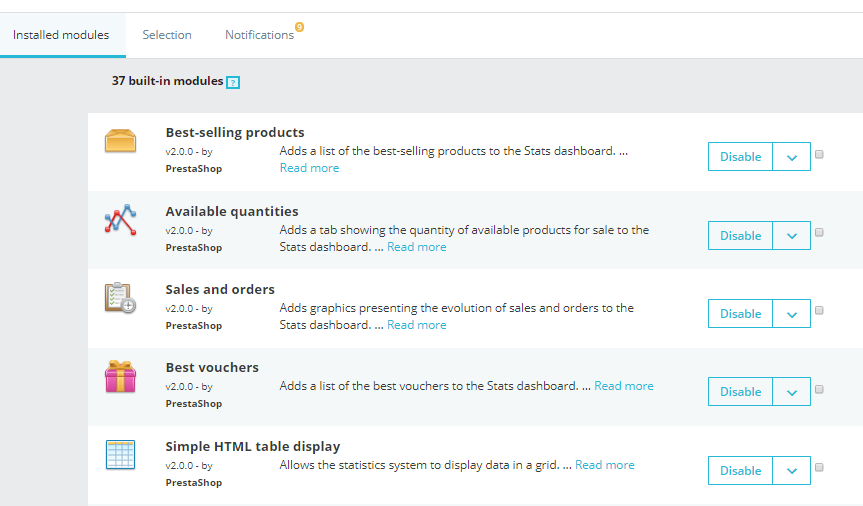
\includegraphics[scale=0.4]{images/modulos.png}
\end{center}

\subsubsection{Diseño}

Funcionalidad que permite llevar todo el tema del diseño de la tienda tanto estético como funcional. Está sectorizado por diseño relacionado con el logo y el tema de la tienda, el contenido del cuerpo de la tienda, del catálogo, las posiciones de los módulos de la página, configuración de imágenes, etc.

\begin{center}
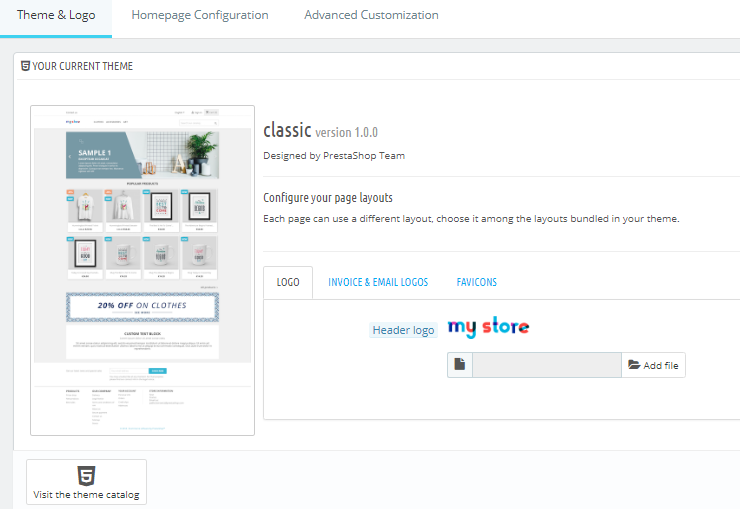
\includegraphics[scale=0.6]{images/diseno.png}
\end{center}

El catálogo de una tienda tanto visualmente como funcionalmente es una de las cosas más importantes de una tienda, sobre todo una tienda online. Por ello Prestashop tiene un catálogo de plantillas ya implementadas de catálogos diseñados que se pueden comprar.
Cualquier información legal o referente a las condiciones de la tienda es algo que el cliente debe de saber, por ello Prestashop tiene una pestaña llamada \textit{páginas} en la cual se le atribuye un nombre a un documento o página que lleva a la información que se quiere dar, sobre la cual profundizaremos más tarde.

\subsubsection{Envio}

En la pestaña de transportistas están las diferentes modalidades de envío. Como pueden ser la recogida en tienda física, el envío mediante Correos Exprés, etc y esta funcionalidad permite añadir o eliminar estas modalidades.
En la pestaña de preferencias se pueden editar las opciones en relación a la empresa que envía los paquetes como la empresa por defecto, ordenar por precio, etc. y también se puede establecer restricciones para los envíos gratis por precio o peso y establecer el precio del envío.

\begin{center}
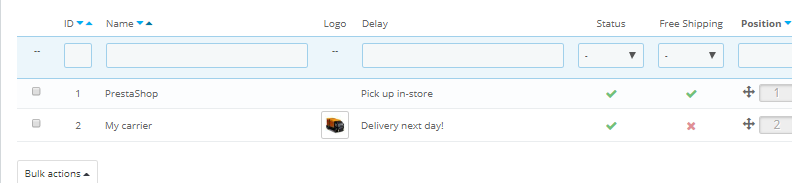
\includegraphics[scale=0.4]{images/envio.png}
\end{center}

\subsubsection{Pagos}

Aquí se encuentra la funcionalidad relacionada con los pagos, algo imprescindible para una tienda.  Si se tienen diferentes métodos de pago, se pueden añadir a la tienda y personalizarlos. Un método de pago se puede restringir a un tipo de moneda o el tipo de perfil del cliente (Visitante, Invitado, Cliente registrado) o por país, funcionalidad que se encuentra en la pestaña de Preferencias.

\begin{center}
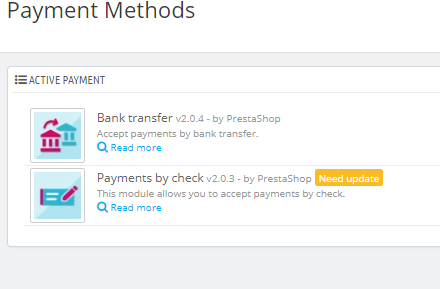
\includegraphics[scale=0.6]{images/payment.png}
\end{center}

\subsubsection{Internacional}

\begin{figure}[h!]
        \raggedright
        \begin{subfigure}[!]{0.4\textwidth} 
            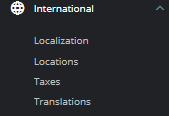
\includegraphics[width=\textwidth]{images/inter.png}
        \end{subfigure}       
        \begin{subfigure}[!]{0.4\textwidth} 
            Función para establecer los ajustes internacionales de la tienda, como país de localización, moneda de pago, idiomas de la tienda, IVA que se aplica al producto (distinto por cada país). Se pueden habilitar zonas (Europa, Asia del este, África, etc) que pueden comprar en nuestra tienda.
        \end{subfigure}
    \end{figure}
    
\begin{center}
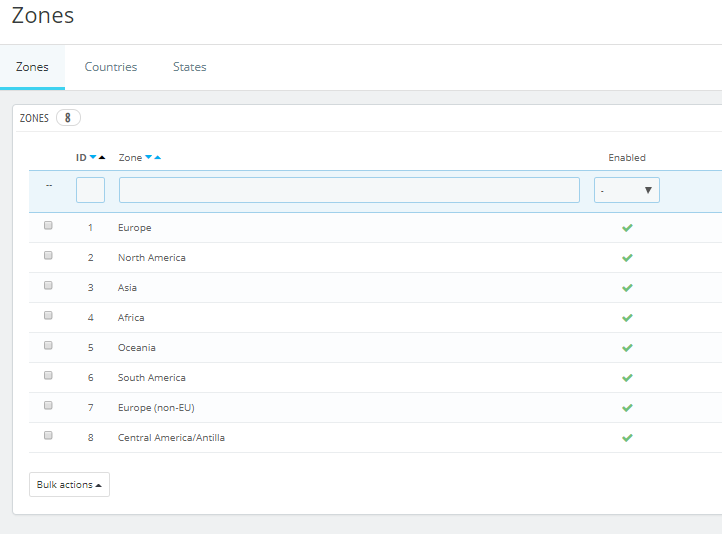
\includegraphics[scale=0.6]{images/zona.png}
\end{center}

\begin{center}
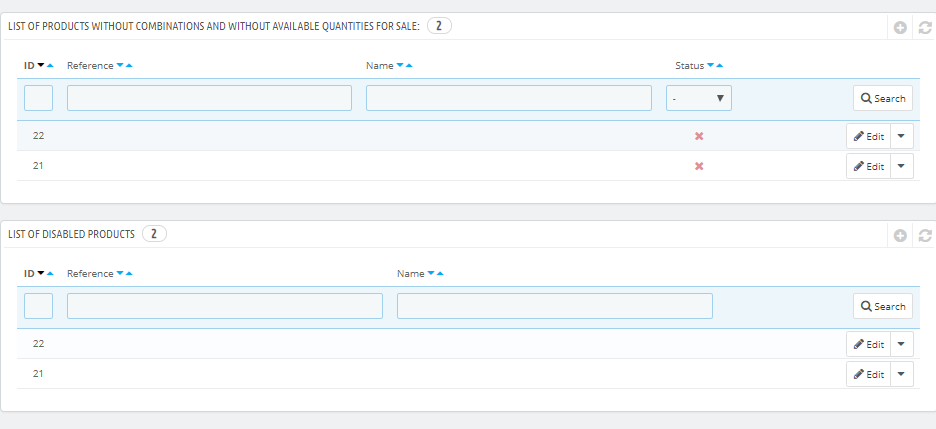
\includegraphics[scale=0.4]{images/lista.png}
\end{center}

\subsubsection{Configuración}

En configuración se pueden modificar los parámetros de la tienda y los parámetros avanzados. En los parámetros de la tienda están los ajustes generales y los ajustes referentes a los pedidos, productos, clientes, contactos, SEO, etc.
Esta funcionalidad es bastante importante, ya que cualquier tienda debe tener certificados SSL, posibilidad de modificar el dominio, importar o exportar datos, etc .

\begin{center}
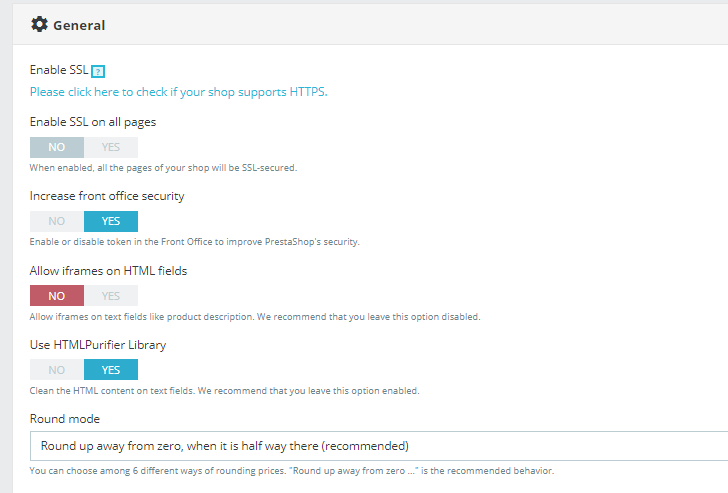
\includegraphics[scale=0.6]{images/conf.png}
\end{center}

En los parámetros avanzados se pueden añadir roles de administrador de la tienda, opciones de email, representación…

\subsection{Creación de la tienda}

En nuestra tienda este cliente, Mary May, ha comprado dos vestidos:

\begin{center}
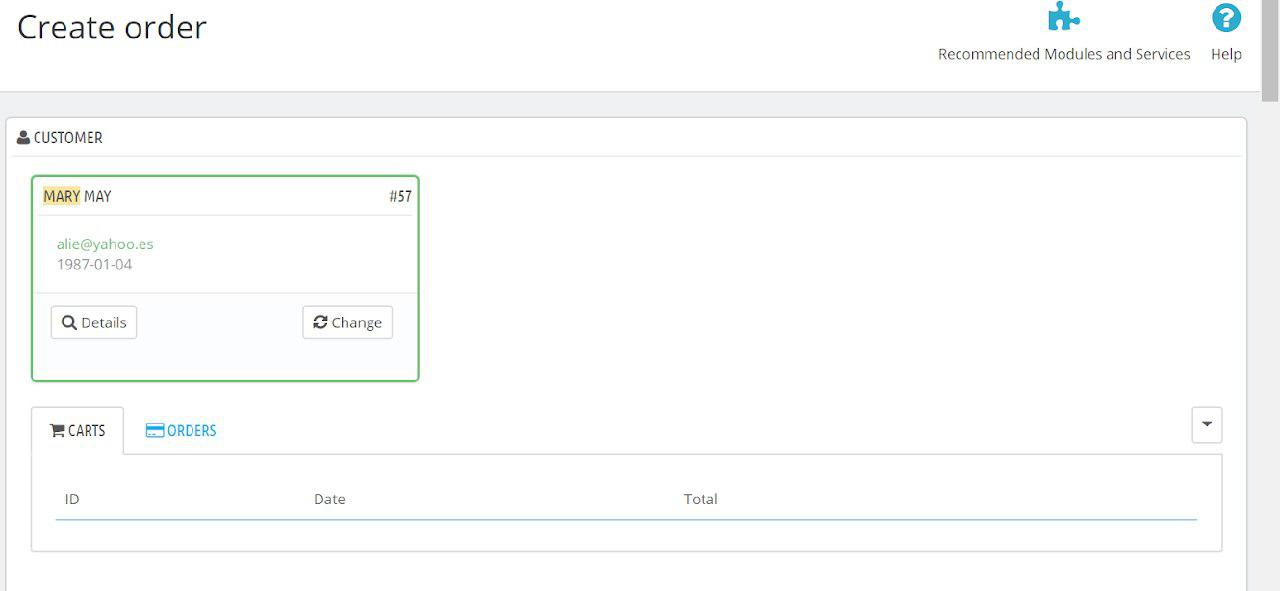
\includegraphics[scale=0.4]{images/order.jpg}
\end{center}

\begin{center}
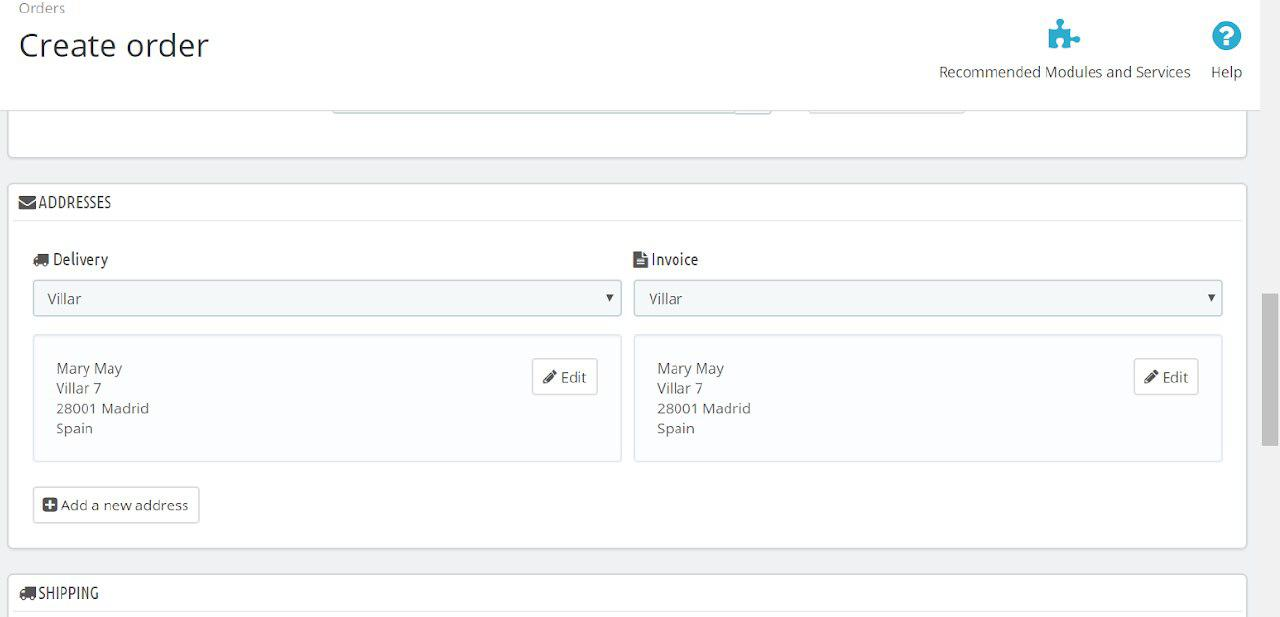
\includegraphics[scale=0.4]{images/order2.jpg}
\end{center}

\begin{center}
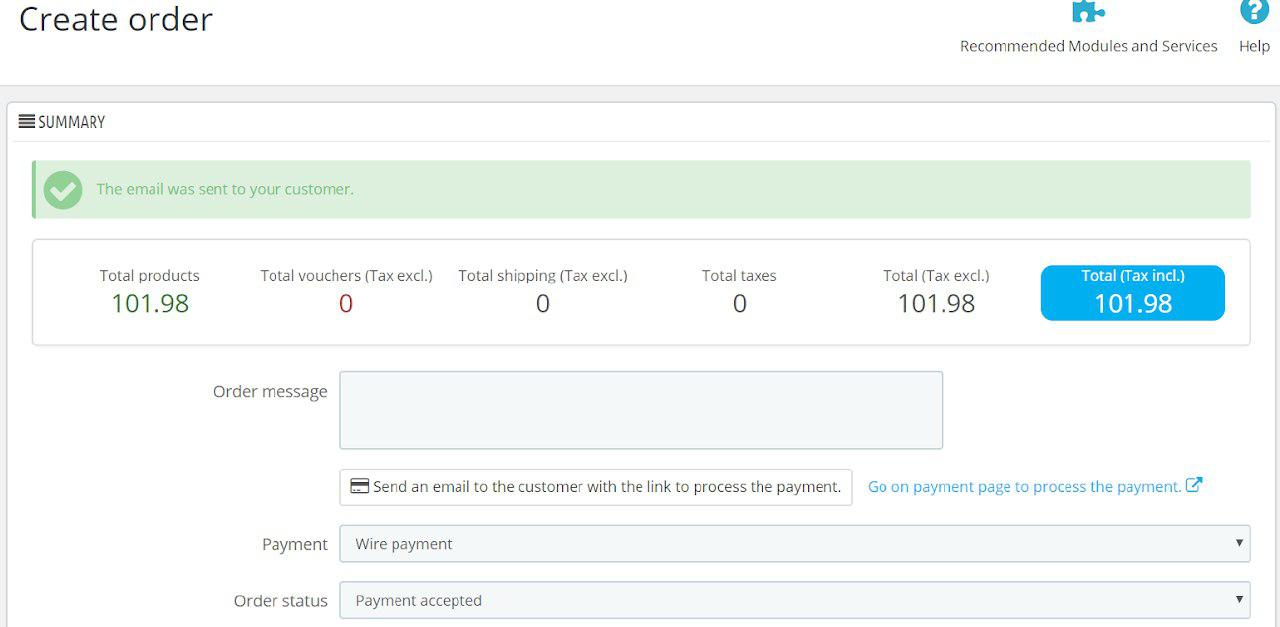
\includegraphics[scale=0.4]{images/order3.jpg}
\end{center}

Pero en el apartado de carrito de compras podemos visualizar que el cliente anterior ha incluido dos vestidos allí, pero todavía no los ha comprado:

\begin{center}
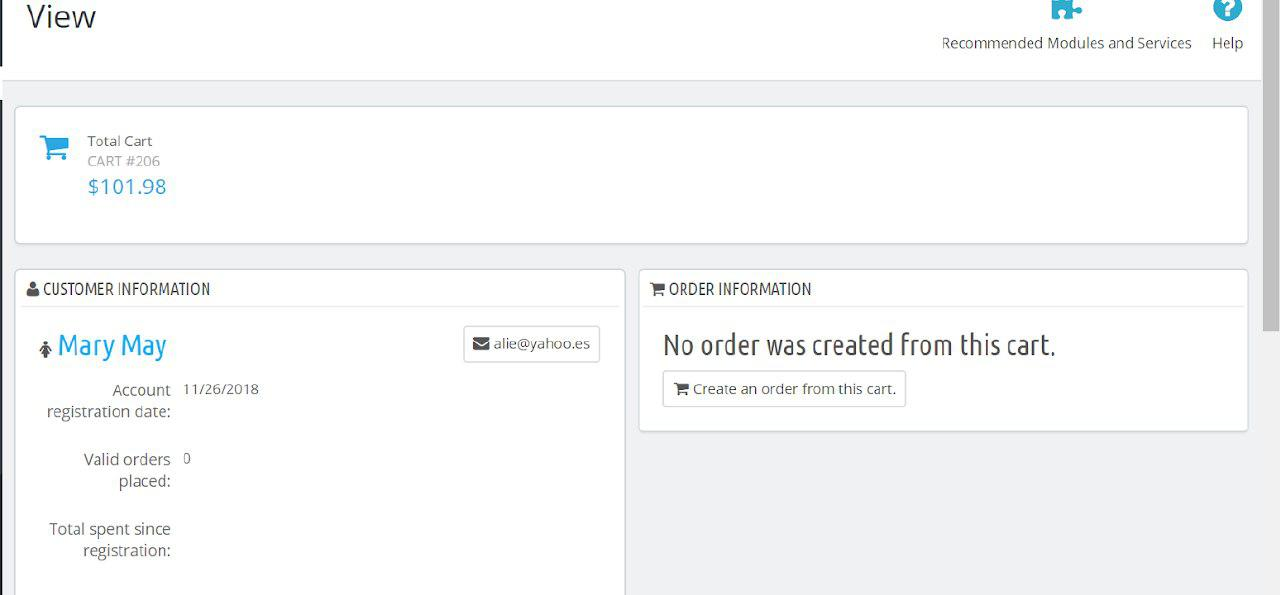
\includegraphics[scale=0.4]{images/order4.jpg}
\end{center}

La vista desde el cliente:

\begin{center}
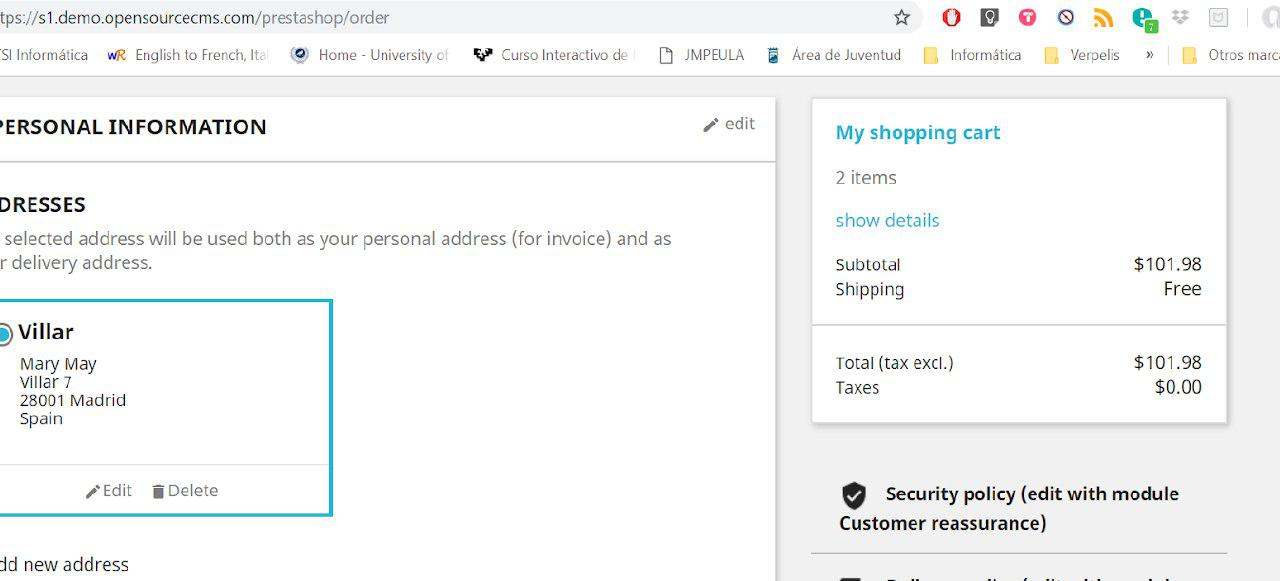
\includegraphics[scale=0.4]{images/order5.jpg}
\end{center}

Hemos añadido un par de productos como este reloj, por ejemplo:

\begin{center}
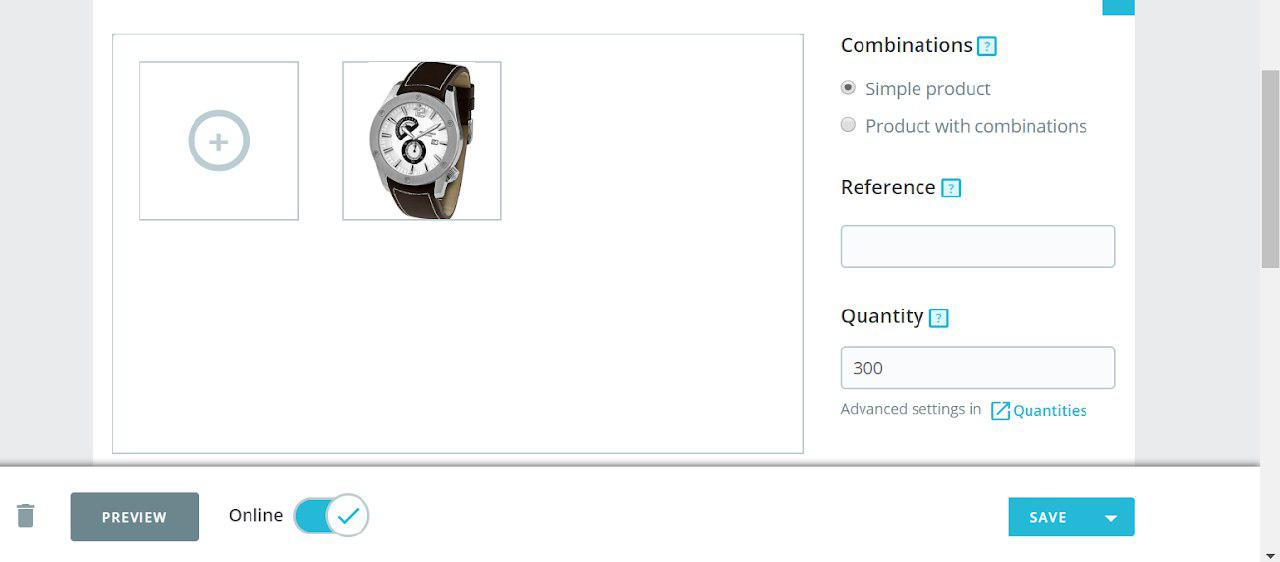
\includegraphics[scale=0.4]{images/order6.jpg}
\end{center}

Lo que vería el cliente (no hemos podido añadir imagen porque salía error):

\begin{center}
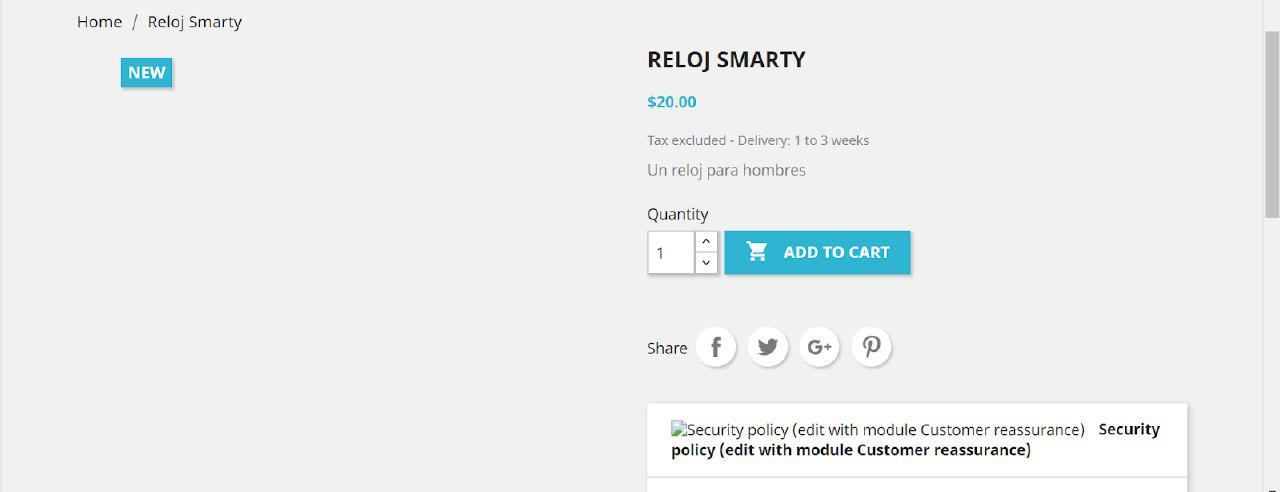
\includegraphics[scale=0.4]{images/order7.jpg}
\end{center}

Hemos creado un par de clientes desde nuestro usuario administrador:

\begin{center}
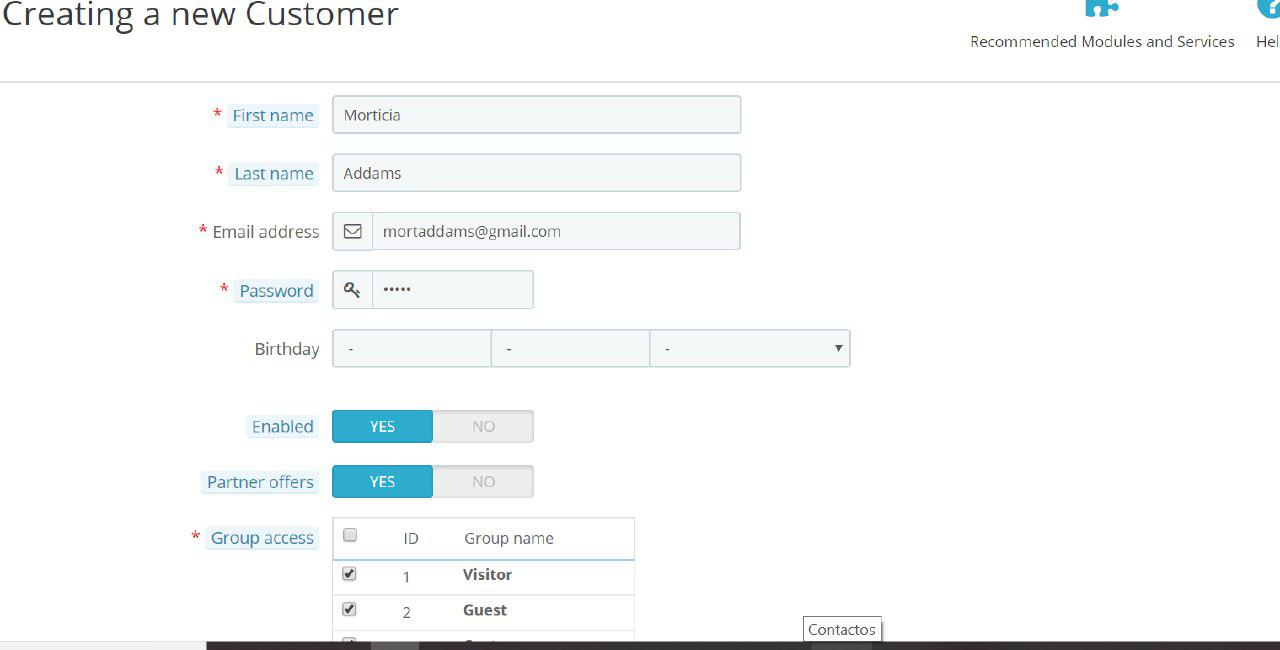
\includegraphics[scale=0.4]{images/order8.jpg}
\end{center}

Y otros más:

\begin{center}
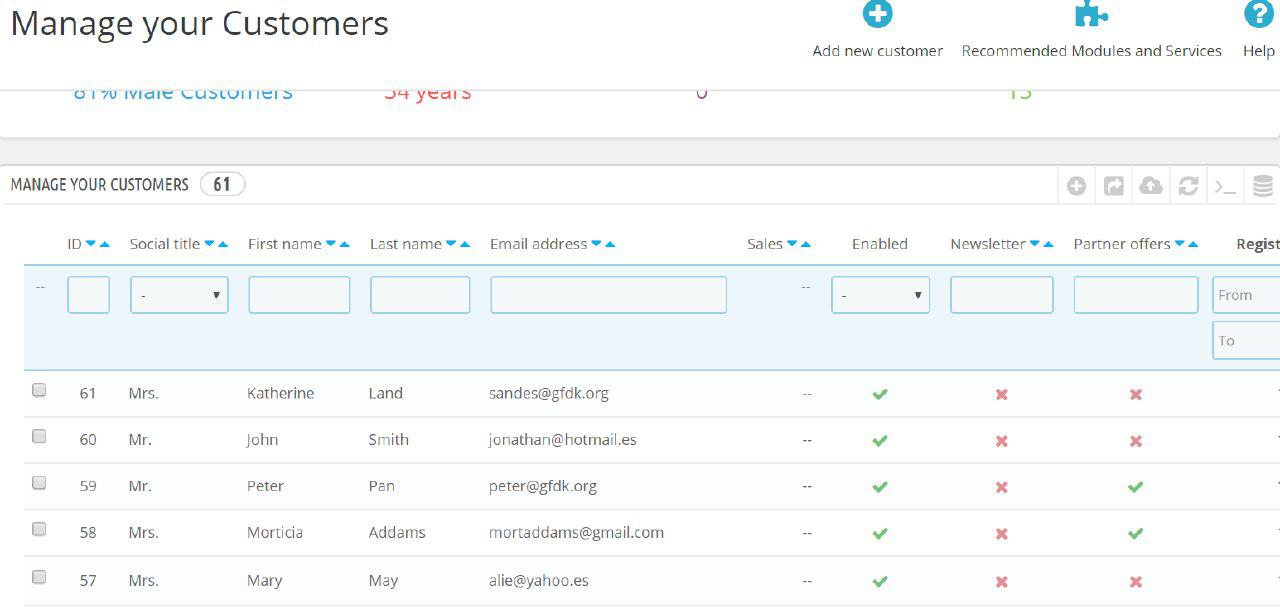
\includegraphics[scale=0.4]{images/order9.jpg}
\end{center}

Como se puede observar podemos quitarles el acceso a algunos usuarios a nuestra tienda, o hacerles que reciban novedades de la tienda en sus correos. También algunos usuarios pueden tener descuento por ser socios. Desde Dirección en Clientes puedes añadir más clientes:

\begin{center}
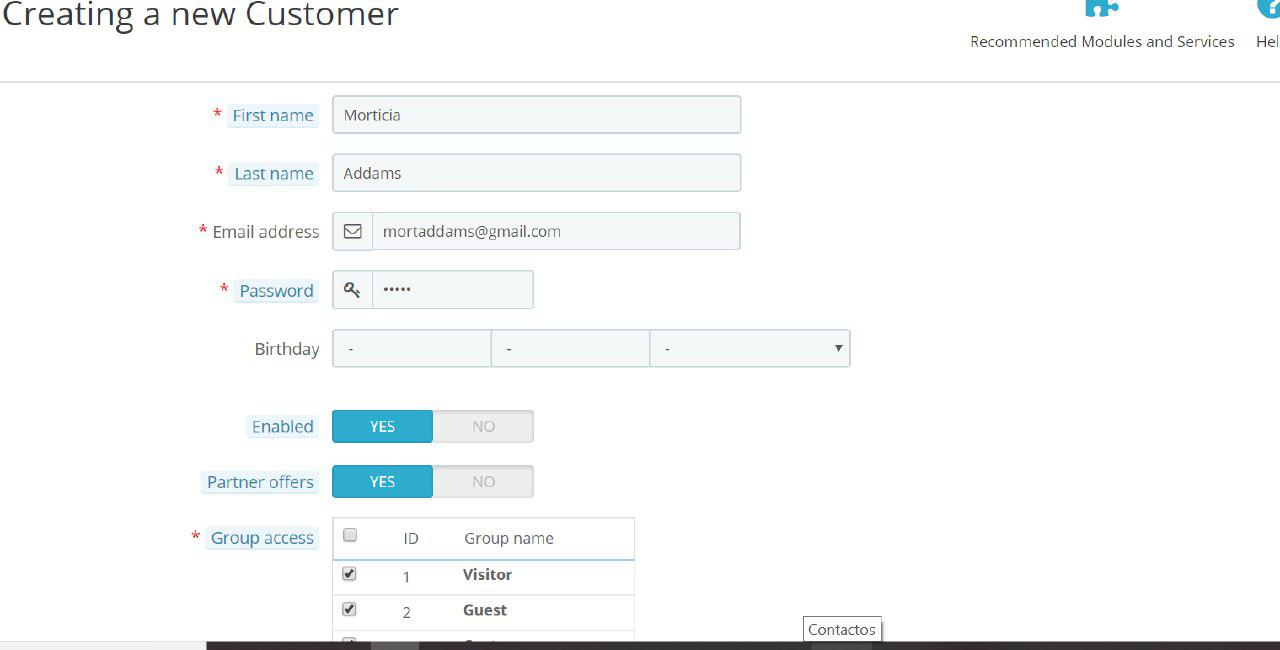
\includegraphics[scale=0.4]{images/order10.jpg}
\end{center}

\section{Relación con la teoría}

\subsection{Control de acceso y seguridad}

\begin{itemize}
\item[-] \textbf{Autenticación}
\end{itemize}

Hay dos partes que deben ser autenticadas: el vendedor (la tienda online) y el cliente.

En el caso del cliente, si está registrado con su información personal en la tienda, al hacer una compra se sabe que el cliente es quien dice ser. Si no está registrado, puede pedir productos como invitado, proporcionando sus datos personales para ello (esta información puede no ser verdadera, pero esto a la tienda no le importa, ya que la tienda recibe el pago y envía el producto, de manera que la transacción consta y abstractamente hay un cliente que ha comprado).

\begin{center}
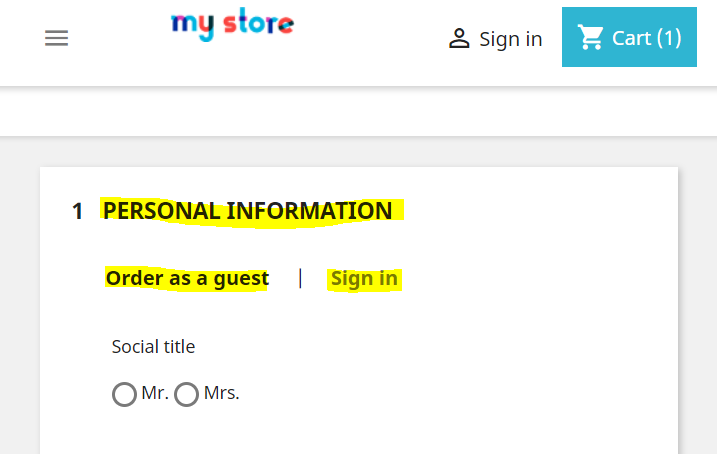
\includegraphics[scale=0.4]{images/autenticacion.png}
\end{center}

En el caso de la tienda online, esta estará certificada con un certificado digital que haga que el navegador considere la web como segura, probando así su autenticidad. Para ello, se debe conseguir un certificado SSL e instalarlo para Prestashop. Luego se configura Prestashop para que trabaje con HTTPS, implementando así \textbf{conexiones seguras}. 

\begin{center}
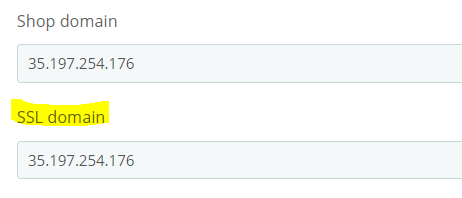
\includegraphics[scale=0.4]{images/auten.png}
\end{center}

\begin{itemize}
\item[-] \textbf{Control de visibilidad}
\end{itemize}

Según el usuario de nuestra tienda, hay diferentes perfiles según la función del usuario.
Si el usuario es un cliente, puede tener el perfil de cliente registrado o cliente invitado, como se mencionó previamente.

Si el usuario es alguien que administra la tienda, tiene el perfil de administrador. Dentro del perfil de administrador hay sub-perfiles, cada cual con una función asignada. Estos sub-perfiles son personalizables, depende de la organización que se encargue de la tienda, puede haber más perfiles, menos y con la función que convenga. Por defecto, Prestashop tiene los perfiles: \textit{SuperAdmin}, \textit{Logistician}, \textit{Translator}, \textit{Salesman}.

\begin{center}
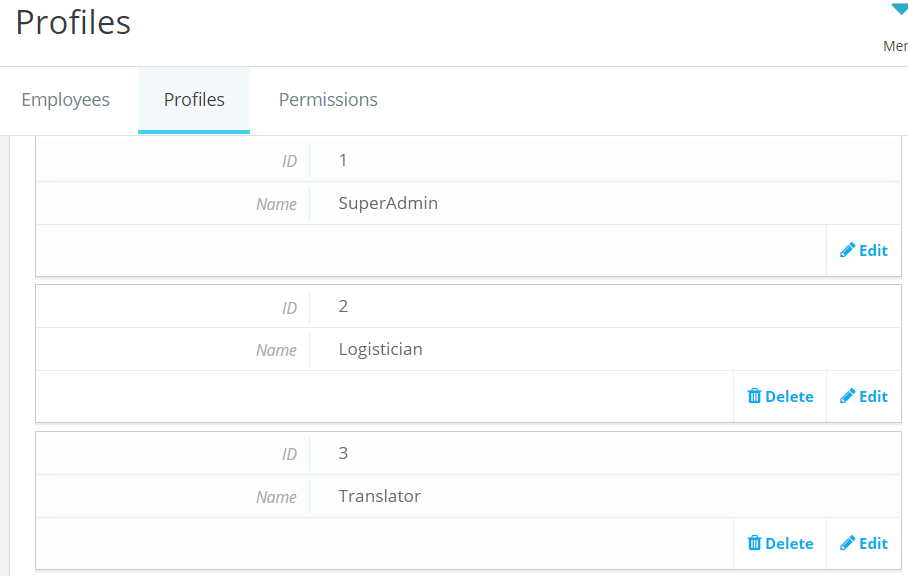
\includegraphics[scale=0.4]{images/profiles.png}
\end{center}

\begin{itemize}
\item[-] \textbf{Protección contra ataques y robos de información}
\end{itemize}

Nuestra tienda online debe ser segura, para ello lo primero es mantener actualizado Prestashop, ya que en cada actualización corregirán vulnerabilidades. También es imprescindible que la tienda disponga de un certificado SSL, que como se menciona previamente, Prestashop permite la instalación de este tipo de certificados (compatible con friendly URL). Otra herramienta para proteger nuestra tienda online es restringir los permisos de la página web (modificando los permisos del fichero .htaccess). 

\subsection{Personalización}

De esto hablaremos más adelante en la memoria, pero como introducción, diremos que es bastante personalizable, pudiendo incluso decir que es uno de sus puntos fuertes.

\subsection{Administración de las búsquedas}

En la configuración de la tienda en la vista de administración de Prestashop se puede configurar las características del motor de búsqueda interno de nuestra tienda. Como por ejemplo, si se introduce el inicio de la palabra que se incluya o no el autocompletar o el peso del indexado de los productos. Si se le quiere dar más importancia al nombre del producto que a la descripción, se le pone un peso mayor, y en caso contrario, menor.

\begin{center}
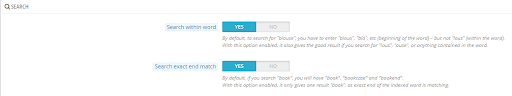
\includegraphics[scale=0.4]{images/search.png}
\end{center}
\begin{center}
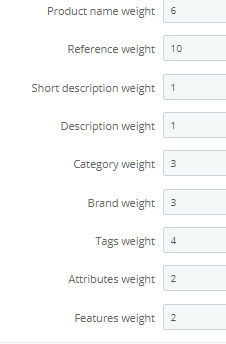
\includegraphics[scale=0.4]{images/weight.png}
\end{center}

Aparte, en el administrador de catálogos, cuando se añade un producto, existe la posibilidad de optimizar la herramienta de búsqueda(SEO).

\subsection{Administración de contenidos}

\begin{figure}[h!]
        \raggedright
        \begin{subfigure}[!]{0.4\textwidth} 
            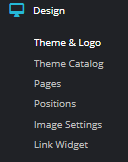
\includegraphics[width=\textwidth]{images/design.png}
        \end{subfigure}       
        \begin{subfigure}[!]{0.7\textwidth} 
            Prestashop proporciona una herramienta de administración de contenidos bastante completa e intuitiva. De manera sectorizada, se puede ir personalizando la tienda.
        \end{subfigure}
    \end{figure}
    
\begin{figure}[h!]
        \raggedright     
        \begin{subfigure}[!]{0.7\textwidth} 
            \begin{itemize}
				\item[\triangleright] Con \texit{Theme&Logo} se puede cambiar el logo de la tienda, el icono asociado al email y el icono asociado a la página que se visualiza                                                     en el navegador. En esta sección también se puede modificar la página principal de la tienda de manera gráfica pulsando el módulo de la página que se quiere cambiar. Por último, hay una customización avanzada en la cual en vez de personalizar el tema de la página, se puede modificar el tema de manera local (HTML/CSS) y luego subirlo.
			\end{itemize}
        \end{subfigure}
        \begin{subfigure}[!]{0.29\textwidth} 
            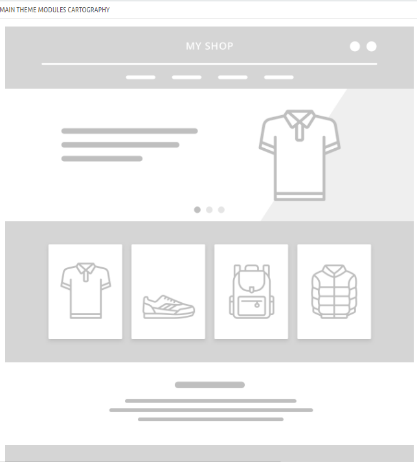
\includegraphics[width=\textwidth]{images/themelogo.png}
        \end{subfigure}  
    \end{figure}
    
\begin{itemize}
\item[\triangleright] Con \textit{Theme&Catalog} se puede comprar y descargar un tema para la visualización del catálogo y personalizar este tema a gusto del administrador/diseñador.
\end{itemize}

\begin{center}
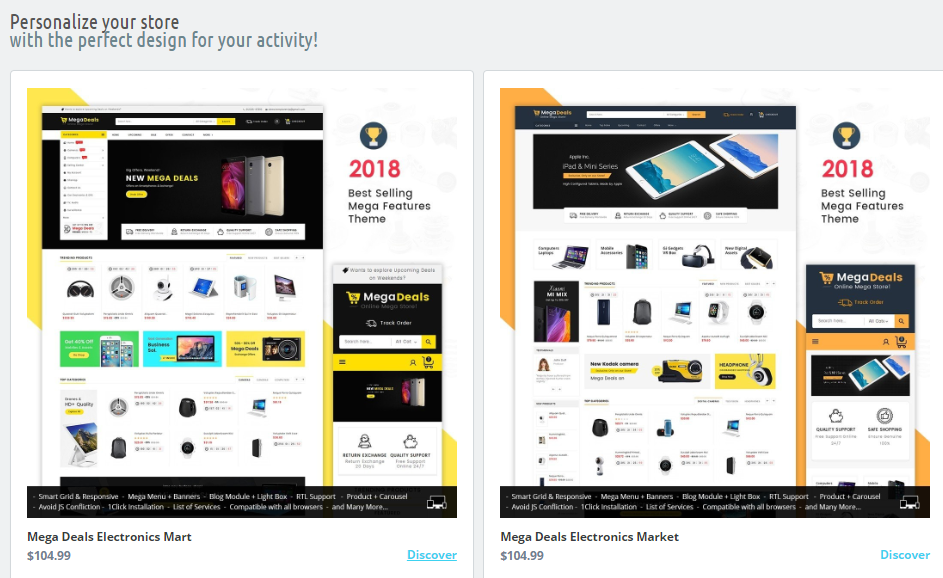
\includegraphics[scale=0.4]{images/themecatalog.png}
\end{center}

\begin{itemize}
\item[\triangleright] Con \textit{Pages} se puede introducir la información que tendría la página que leería el visitante de la tienda y posible comprador si pulsa el enlace que redirecta a esa página. Por ejemplo, cuando hay que aceptar los términos de uso o la ley de protección de datos, hay que decirle al cliente cómo puede acceder a esos documentos, normalmente se hace mediante un enlace.
\end{itemize}

\begin{center}
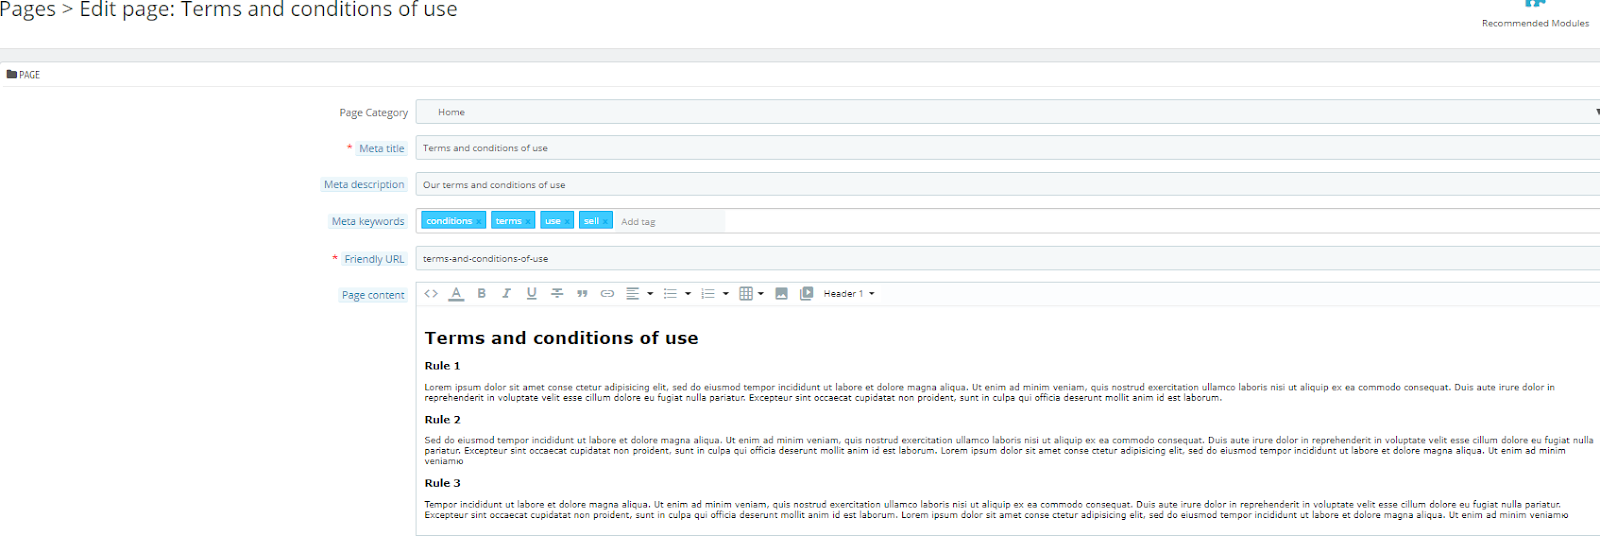
\includegraphics[scale=0.25]{images/pages.png}
\end{center}

\begin{itemize}
\item[\triangleright] \textit{Positions} permite establecer la posición de cada módulo de la página de nuestra tienda. Por ejemplo, el módulo de Navegación va después del módulo donde se encuentra el menú y contiene la selección del idioma de la página, la moneda, Iniciar sesión, carrito, etc.
\end{itemize}

\begin{center}
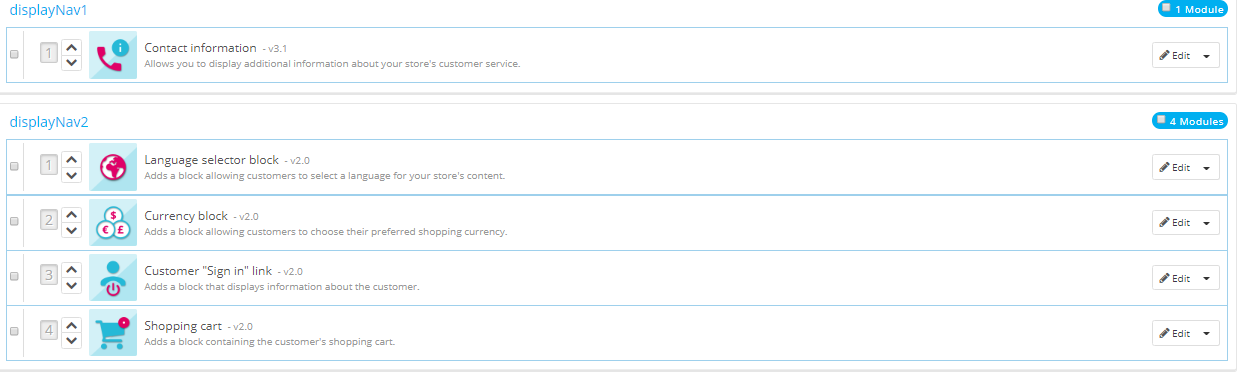
\includegraphics[scale=0.3]{images/positions.png}
\end{center}

\begin{itemize}
\item[\triangleright] \textit{Image Settings} permite personalizar la configuración de las imágenes (formato de imagen, tamaño de compresión, tamaño de la imagen, selección de resolución) y se pueden crear distintas configuraciones y guardarlas, para que en un futuro se puedan usar configuraciones ya creadas.
\end{itemize}

\begin{itemize}
\item[\triangleright] \textit{Link Widget} sirve para introducir widgets en la página según la posición conveniente pudiendo enlazar contenidos ya creados de la página.
\end{itemize}

\subsection{Administración de catálogos}

Prestashop en la barra lateral tiene un administrador de catálogos, el cual tiene distintas herramientas:

\begin{figure}[h!]
        \raggedright
        \begin{subfigure}[!]{0.2\textwidth} 
            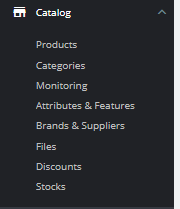
\includegraphics[width=\textwidth]{images/catalog.png}
        \end{subfigure}       
        \begin{subfigure}[!]{0.7\textwidth} 
            \begin{itemize}
\item[\triangleright] \textibf{Productos:} Se pueden añadir o eliminar productos, de manera personalizada(estableciendo visibilidad, condiciones, subiendo archivos o los propios clientes pueden personalizar el producto introduciendo un texto o imágenes).
\end{itemize}            
        \end{subfigure}
    \end{figure}
    
\begin{itemize}
				\item[\triangleright] \textbf{Categorías:} Se pueden añadir o eliminar categorías, y cuando se añaden se puede elegir el grupo que puede tener acceso a esa categoría. Por ejemplo, un cliente puede ver la categoría pero un invitado no.
			\end{itemize}

\begin{itemize}
				\item[\triangleright] \textbf{Atributos y Características:} Herramienta de personalización de los elementos del catálogo mediante atributos (talla de la camiseta, color, dimensiones, etc.) y características (material, marca, etc.).
			\end{itemize}

\begin{itemize}
				\item[\triangleright] \textbf{Marcas y Proveedores:} Proporciona la integración con subsistemas de Almacén, ya que tiene información de los proveedores y las marcas de los productos que se comercializan en nuestra tienda.
			\end{itemize}
			
			\begin{itemize}
				\item[\triangleright] \textbf{Descuentos:} Proporciona integración con subsistemas de gestión comercial. Ya que si a un producto se le aplican descuentos, esto luego se refleja en las ventas.
			\end{itemize}
			
			\begin{itemize}
				\item[\triangleright] \textbf{Stocks:} Proporciona integración con el subsistema de Almacén, ya que al contar el número de productos que están disponibles y estar automatizado facilita la tarea.
			\end{itemize}
			
\subsection{Pago y Compra}

Prestashop tiene implementadas múltiples herramientas de compra y pago:

\begin{itemize}
				\item[\triangleright] \textbf{Carrito de la compra:} Desde el inicio de la configuración de la tienda, se tiene un carrito de la compra básico el cual se puede personalizar, por ejemplo, usando módulos, como \href{https://addons.prestashop.com/en/emails-notifications/26203-browser-tab-notification-favicon.html?utm_source=back-office&utm_medium=push-addons&utm_campaign=back-office-EN&utm_content=download}{este}.
				\begin{center}
				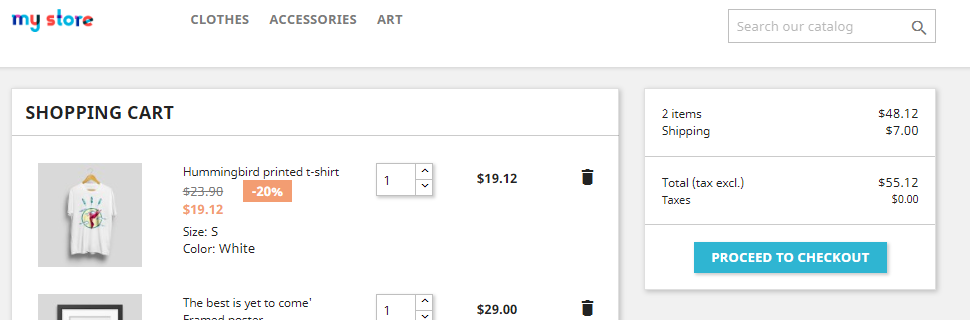
\includegraphics[scale=0.4]{images/carrito.png}
				\end{center}
			\end{itemize}

\begin{itemize}
				\item[\triangleright] \textbf{Wishlist:} Al comenzar a usar Prestashop, las listas de productos deseados no están implementadas, pero si se quieren añadir, Prestashop dispone de módulos útiles que permiten disponer de esta herramienta en nuestra tienda.\\
				\href{https://addons.prestashop.com/en/wishlist-gift-card/26835-wishlist-buy-later-save-for-later.html?utm_source=back-office&utm_medium=push-addons&utm_campaign=back-office-EN&utm_content=download}{Adavanced Wishlist Module.}\\
				\href{https://addons.prestashop.com/en/wishlist-gift-card/26835-wishlist-buy-later-save-for-later.html?utm_source=back-office&utm_medium=push-addons&utm_campaign=back-office-EN&utm_content=download}{Wishlist Buy Later (safe for later) Module.}
				\begin{center}
				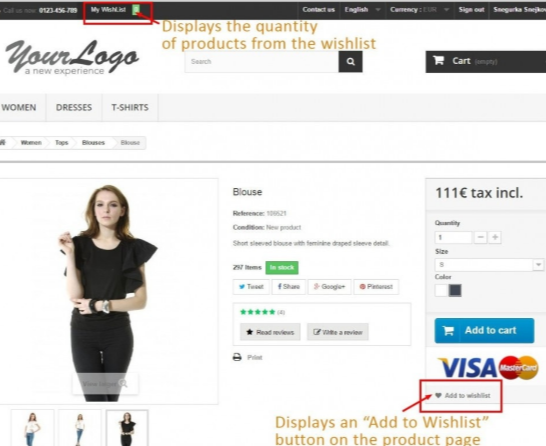
\includegraphics[scale=0.4]{images/wishlist.png}
				\end{center}				
			\end{itemize}
			
			\begin{itemize}
				\item[\triangleright] \textbf{Devoluciones:} Dentro del menú lateral de Prestashop en la visión de administrador, en Servicio al Cliente, hay una pestaña que trata el tema de las devoluciones de productos a los clientes. Se puede permitir la devolución o no en la tienda y el número límite de días.
				\begin{center}
				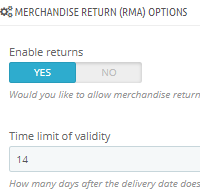
\includegraphics[scale=0.4]{images/devoluciones.png}
				\end{center}
			\end{itemize}
			
			\begin{itemize}
				\item[\triangleright] \textbf{Métodos de pago:} Inicialmente solo de disponen de dos métodos de pago disponibles en nuestra tienda: Pago por transferencia Bancaria y Pago por cheque. 
				\begin{center}
				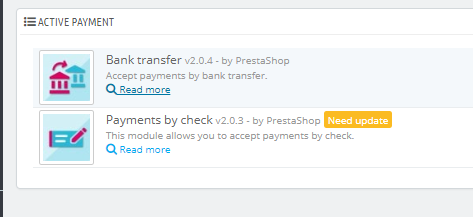
\includegraphics[scale=0.4]{images/pagos.png}
				\end{center}
				Usualmente se suele utilizar el método de pago por tarjeta bancaria, así que, si queremos incluir ese método de pago en nuestra tienda, hay que utilizar un módulo, como por ejemplo: \href{https://addons.prestashop.com/en/other-payment-methods/18635-wk-payment-by-credit-check.html&utm_source=back-office&utm_medium=search&utm_campaign=back-office-EN&utm_content=download}{WK Payment By Credit Check Module}.
				
Y para el pago seguro se puede usar un módulo REDSYS con integración, que certifica un pago seguro, y una devolución segura dando seguridad a las transacciones monetarias. Por ejemplo, \href{https://addons.prestashop.com/es/pago-tarjeta-carteras-digitales/16398-redsys-tpv-completo-pago-seguro-devoluciones.html}{Módulo REDSYS TPV COMPLETO}.
			\end{itemize}
			
\subsection{Administración del flujo de trabajo}
La administración de pedidos incluye la administración del flujo de trabajo.

\begin{center}
	\includegraphics[scale=0.25]{images/flujo.png}
\end{center}

Donde se tiene al cliente y al vendedor, y los procesos del pedido.

\subsection{Notificación de eventos}

Hay un sistema de notificaciones tanto para clientes como para el vendedor, ya que ambos necesitan ser notificados. Para ello, se puede utilizar un módulo, como por ejemplo, \href{https://addons.prestashop.com/es/emails-notificaciones/22787-alertas-notificaciones-sms-email-y-voz-afilnet.html}{Módulo de alertas/Notificaciones} y ya se tiene la funcionalidad de notificaciones.

\subsection{Colaboración y negociación}

Si los clientes pueden comentar los productos y evaluarlos en nuestra tienda, puede existir tanto una comunicación de cliente a cliente o entre clientes y empleados de nuestra tienda. Por ello conviene tener un módulo, como por ejemplo,\href{https://addons.prestashop.com/es/comentarios-clientes/22373-comentarios-avanzados-con-fotos-google-rich-snippets.html}{Módulo de comentarios avanzados con fotos}.

\section{Personalización e integración}

\subsection{Personalización}

Una vez que un cliente realiza una compra, se registra su información (compra y personal), de manera que en la pestaña de administración de clientes se puede ver un resumen de los datos generales de los clientes estadíscticamente.

En la pestaña de stats del menú lateral de la vista de administración de Prestashop hay una serie de estadísticas que muestran las mejores categorías de la tienda, los mejores clientes, los mejores proveedores, el navegador que usan el cliente cuando compran en nuestra página, las palabras que usan en un buscador para encontrar nuestra página, etc. Esta información se puede usar para personalizar la tienda según esta información obtenida, como hacer una característica especial para un navegador que sea más usado por los clientes de la tienda, cambiar palabras clave según la búsqueda de los clientes en los motores de búsqueda, etc. Y de manera más directa (marketing one-to-one) según la información de las compras de clientes concretos, cogiendo a los mejores, medios y peores se pueden hacer ofertas personalizadas para obtener beneficio y aumentar la fidelidad del cliente para retenerlo más tiempo.

\begin{center}
\includegraphics[scale=0.5]{images/personalizacion.png}
\end{center}

Cuando un cliente visualiza un producto para su posible compra, existe la posibilidad de compartirlo por redes sociales, otra manera de obtener información (más subjetiva) de los clientes.
Las cookies, mientras se cumpla la ley de cookies de la Unión Europea que obliga a todas las páginas web a informar y obtener el consentimiento del visitante de la utilización de las cookies en la página web. De esta manera, nuestra página puede obtener información de cada cliente o potencial cliente sobre la actividad anterior de su navegador, pudiendo mostrar publicidad, ofertas, etc. a medida para los clientes.

\subsection{Integración}

Como muchas de las funcionalidades disponibles, es posible la integración con otros CRM, ERP, software de facturación y otros tipos de software que complementen la actividad del negocio.

Todos estos módulos los podremos buscar en la página oficial de Prestashop. Los módulos de integración destacados son:

\begin{center}
\includegraphics[scale=0.4]{images/integracion.png}
\end{center}

Cabe destacar que solo un módulo es gratuito, y es el de integración con Sage 50Cloud por ser socio oficial de Prestashop.

\section{Conclusiones}

Al trabajar con prestashop estaremos optimizando en gran medida los recursos humanos, ya que casi en su totalidad estaremos reutilizando módulos que ya han creado otras personas previamente y además no necesitaremos un amplio personal para que programe la tienda online.

Esto provocará beneficios a corto plazo para la empresa, ya que se encargará y entregará un producto, en este caso, una página web, con la mayor brevedad y eficacia posible
Otra de la ventajas es que detrás de Prestashop hay una gran comunidad. Por lo que si surgen dudas o problemas se podrán encontrar soluciones rápido, ( o si se trata de  personalización)  resumiendo,  es más conocido en el mundo empresarial. 

Por contraposición al desconocer en parte el contenido total de los módulos con los que estamos trabajando, a veces no nos será posible personalizar tanto las páginas como queramos, lo cual podrá no agradar por completo a los clientes, aunque se le entregue el producto en fecha.

Luego la estrategia de marketing y de ventas para poder obtener la mayor cantidad de beneficios será orientar a buscar un conjunto de clientes cuanto mayor mejor, que deseen tener tiendas online sencillas, sin gran detalle ni personalización pero que las quieran rápido.

La gestión de almacén en este caso, será el tiempo del que dispondrán cada uno de los programadores y/o encargados de realizar una tienda online con prestashop para realizar dicha página.

De forma general, prestashop nos ofrecerá un conjunto de herramientas y módulos prediseñados que, sin un alto nivel en conocimientos de programación podremos crear una tienda online útil y funcional, sólo que esta será de carácter general y posiblemente poco personalizada.


\begin{thebibliography}{9}

\bibitem{SSL} \textit{Certificado SSL para Prestashop}, \url{https://guiadev.com/certificado-ssl-para-prestashop/}.
\bibitem{Seguridad} \textit{Seguridad y fiabilidad en Prestashop}, \url{https://www.prestashop.com/forums/topic/237776-sobre-seguridad-y-confianza/}.
\bibitem{htaccess} \textit{Información y usos del fichero .htaccess}, \url{https://ticket.cdmon.com/es/support/solutions/articles/7000006237-informaci\%C3\%B3n-y-usos-del-fichero-htaccess}.
\bibitem{cookie} \textit{Cookies}, \url{https://es.wikipedia.org/wiki/Cookie_(inform\%C3\%A1tica)}.
\bibitem{cookies} \textit{Legislación europea de cookies}, \url{https://privacypolicies.com/blog/eu-cookie-law/#what-is-the-eu-cookie-legislation}.
\bibitem{linkwidget} \textit{Link Widget en Prestashop}, \url{https://zemez.io/prestashop/support/how-to/prestashop-1-7-x-manage-link-widget/}.
\bibitem{wishlist} \textit{Lista de deseos en Prestashop}, \url{https://addons.prestashop.com/en/wishlist-gift-card/26835-wishlist-buy-later-save-for-later.html?utm_source=back-office&utm_medium=push-addons&utm_campaign=back-office-EN&utm_content=download}.
\bibitem{wishlistcard} \textit{Lista de deseos avanzada en Prestashop}, \url{https://addons.prestashop.com/en/wishlist-gift-card/23903-advanced-wishlist.html&utm_source=back-office&utm_medium=search&utm_campaign=back-office-EN&utm_content=download}.
\bibitem{pagos} \textit{Pago por tarjeta en Prestashop}, \url{https://addons.prestashop.com/en/other-payment-methods/18635-wk-payment-by-credit-check.html&utm_source=back-office&utm_medium=search&utm_campaign=back-office-EN&utm_content=download}.
\bibitem{devoluciones} \textit{Pago seguro y devoluciones}, \url{https://addons.prestashop.com/es/pago-tarjeta-carteras-digitales/16398-redsys-tpv-completo-pago-seguro-devoluciones.html}.
\bibitem{comentarios} \textit{Comentarios con fotos}, \url{https://addons.prestashop.com/es/comentarios-clientes/22373-comentarios-avanzados-con-fotos-google-rich-snippets.html}.
\bibitem{funcionalidades} \textit{Funcionalidades de Prestashop}, \url{https://www.prestashop.com/es/funcionalidades}.
\bibitem{notificaciones} \textit{Notificaciones}, \url{https://addons.prestashop.com/es/emails-notificaciones/22787-alertas-notificaciones-sms-email-y-voz-afilnet.html}.
\bibitem{integracion} \textit{Integración con Prestashop}, \url{https://addons.prestashop.com/es/452-integracion-con-crm-erp}.
\bibitem{enlace} \textit{texto}, \url{http://doc.prestashop.com/plugins/servlet/mobile#content/view/54263818}

\end{thebibliography}



\end{document}